\begin{frame}[hasprev=false, hasnext=true]
\label{example:therac-25}
\frametitle{Therac-25}
\framesubtitle{Description}

\begin{itemize}
	\item Therac-25 was a computerized radiation therapy machine produced
	after the Therac-20 units.

	\item The machine offered two modes of radiation therapy:
	\begin{itemize}
		\item direct electron-beam therapy,

		\item megavolt X-ray therapy, which delivered X-rays produced by
		colliding high-energy (25 MeV) electrons into a target.
	\end{itemize}
\end{itemize}

\begin{figure}
	\centering
	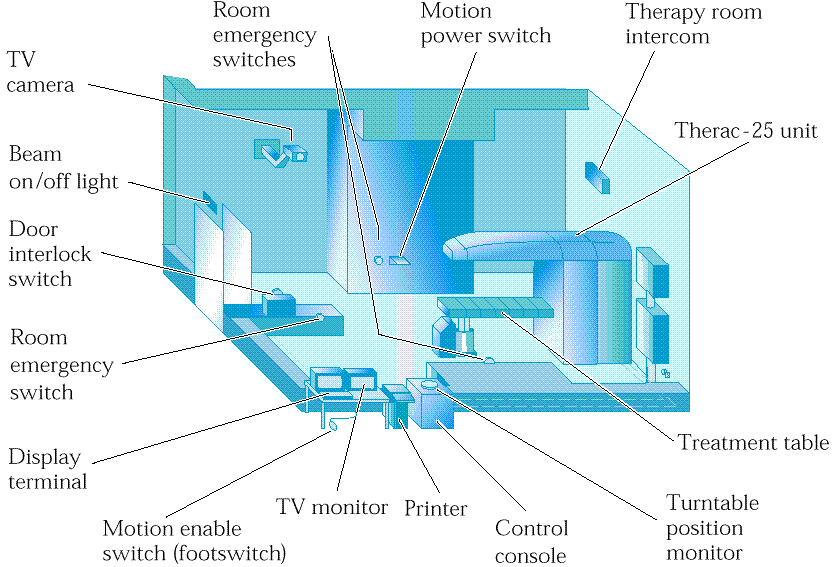
\includegraphics[width=5cm]{aux/examples/therac-25/therac-25}
\end{figure}
\end{frame}



\begin{frame}[hasprev=true, hasnext=true]
\frametitle{Therac-25}
\framesubtitle{Description}

\begin{itemize}
	\item Therac-20 employed independent protective circuits and mechanical
	interlocks to protect against overdose.

	\item Therac-25 relied more heavily on software.

	\item FDA approved Therac-25 as pre-market equivalence to Therac-20
	(even though the safety mechanisms were moved into the software, a
	major change from previous version of the machine.)
\end{itemize}
\end{frame}


\begin{frame}
\frametitle{Therac-25}
\framesubtitle{Problem}

\begin{itemize}
	\item The machine massively overdosed patients at least six times
	between June 1985 and January 1987.
	\begin{itemize}
		\item Each overdose was several times the normal therapeutic dose.

		\item The overdose resulted in the patient's severe injury or even
		death.
	\end{itemize}
\end{itemize}

\begin{figure}
	\centering
	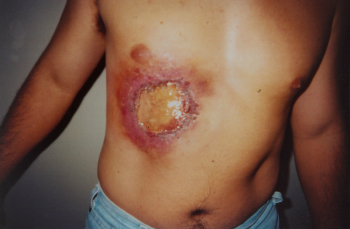
\includegraphics{aux/examples/therac-25/radiation-burn}
\end{figure}

\end{frame}


\begin{frame}
\frametitle{Therac-25}
\framesubtitle{Diagnostic}

\begin{itemize}
	\item The accidents occurred when:
	\begin{enumerate}
		\item \textbf{High-power} electron beam was activated instead of the
		intended \textbf{low power} beam, and
		\item beam spreader plate \textbf{not} rotated into place.
	\end{enumerate}

	\item The machine's software did not detect that this had occurred,
	and therefore did not prevent the patient from receiving a
	potentially lethal dose of radiation.
\end{itemize}
\end{frame}


\begin{frame}
\frametitle{Therac-25}
\framesubtitle{Diagnostic}

\begin{itemize}
	\item The failure only occurred when a particular nonstandard sequence of
	keystrokes was entered on the VT-100 terminal which controlled Therac-25.
\end{itemize}

\begin{figure}
	\centering
	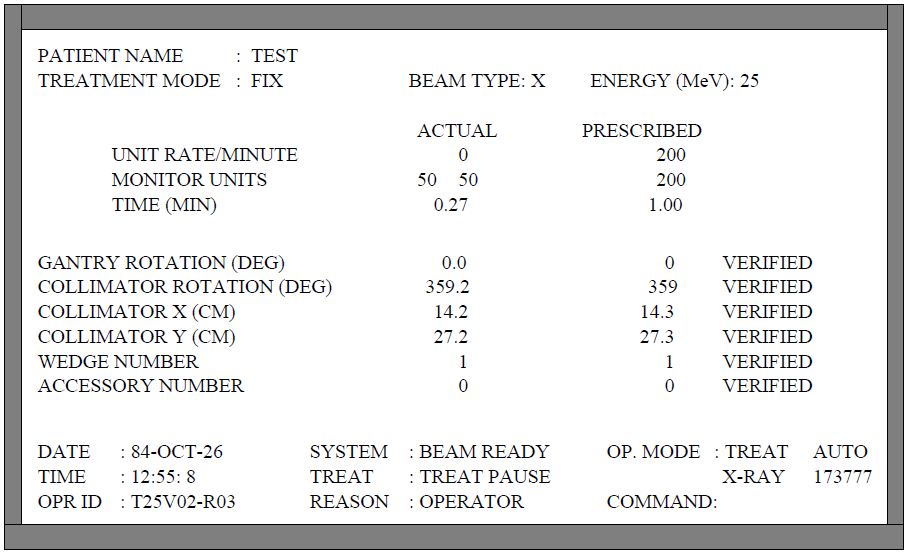
\includegraphics[width=7cm]{aux/examples/therac-25/therac-25-ui}
\end{figure}
\end{frame}


\begin{frame}
\frametitle{Therac-25}
\framesubtitle{Diagnostic}

\begin{itemize}
	\item The primary reason should be attributed to the bad software
	design and development practices and not explicitly to several coding
	errors that were found.
	\begin{itemize}
		\item The equipment control task did not properly synchronize with
		the operator interface task, so that race conditions occurred if
		the operator changed the setup too quickly.

		\item AECL had never tested the Therac-25 with the combination of
		software and hardware until it was assembled at the hospital.
	\end{itemize}
\end{itemize}
\end{frame}



\begin{frame}[hasprev=true, hasnext=false]
\frametitle{Therac-25}
\framesubtitle{Solution}

\begin{itemize}
	\item First suggested solution (proposed by the manufacturer):
	\begin{itemize}
		\item Change in operating procedures:
		\begin{itemize}
			\item The key used for moving the cursor back through the
			prescription sequence (i.e., cursor "UP" inscribed with an upward
			pointing arrow) must not be used for editing or any other purpose.

			\item To avoid accidental use of this key, the key cap must be
			removed and the switch contacts fixed in the open position with
			electrical tape or other insulating material.
		\end{itemize}
	\end{itemize}

	\item After several years of troubleshooting, the final solution was
	comprised of numerous software fixes, the installation of independent,
	mechanical safety interlocks, and a variety of other safety related
	changes.
\end{itemize}

\end{frame}